\documentclass[11pt]{article}
\usepackage[fontsize = 12pt]{scrextend}
\usepackage{multicol}
\usepackage{multirow}
\usepackage{savesym}
\usepackage{hyperref}
\usepackage{amsmath}
\usepackage{algorithm}
\usepackage{algorithmic}
\usepackage{paralist}
\usepackage{float}
\usepackage{bm}
\usepackage[shortlabels]{enumitem}
\usepackage[bb=px]{mathalpha}
\usepackage[a4paper, margin=1in]{geometry}
\usepackage[dvipsnames]{xcolor}
\usepackage{tikz}
\newtheorem{theorem}{Theorem}
\usetikzlibrary{shapes,backgrounds}
\usetikzlibrary{positioning}
\title{SDS 383C - Statistical Modeling 1: Homework 4}
\author{Rahul Nandakumar \\ Graduate Student, ORIE Program (E-ID: rn9355)}
\date{November 9, 2022}
\begin{document}
\maketitle
\noindent \emph{1.}\\ \\
\textbf{Solution:} Given a normal likelihood  model, the likelihood function is given by
\begin{equation}
  \nonumber
  \begin{aligned}
    f(y \text{ } | \text{ } \mu, \sigma^2) & = \frac{1}{\sqrt{2 \pi} \sigma}\text{exp}\bigg(\frac{-1}{2 \sigma^2}(y - \mu)^2 \bigg)\\
    p(y_{1:n} \text{ } | \text{ } \mu, \sigma^2) & = \prod_{i = 1}^{n}\frac{1}{\sqrt{2 \pi} \sigma}\text{exp}\bigg(\frac{-1}{2 \sigma^2}(y_{i} - \mu)^2 \bigg)\\
    & \propto (\sigma^2)^{-n/2}\text{exp}\bigg(\frac{-1}{2 \sigma^2}\big((n-1)s^2 + n(\bar{y} - \mu)^2\big)\bigg)
  \end{aligned}
\end{equation}
The pdf of an NIG Distribution is given by,
\begin{equation}
  \nonumber
  f(x, \sigma^{2} \text{ }|\text{ } \mu, \lambda, \alpha, \beta) = \frac{\sqrt{\lambda}}{\sqrt{2 \pi} \sigma}\frac{\beta^\alpha}{\Gamma(\alpha)}\bigg(\frac{1}{\sigma^{2}}\bigg)^{\alpha + 1} \text{exp}\bigg(-\frac{2 \beta + \lambda(x - \mu)^{2}}{2 \sigma^2}\bigg)
\end{equation}
The a-priori NIG prior on $\mu, \sigma^2$ is given by,
\begin{equation}
  \nonumber
  \begin{aligned}
    p(\mu, \sigma^2) & =  \text{NIG}(\mu_{0}, \sigma_{0}^{2}\ \kappa_{0}, v_{0}, \sigma_{0}^{2})\\
  \end{aligned}
\end{equation}
Here, comparing to the original pdf of NIG Distribution, we can see that
\begin{equation}
  \nonumber
  \begin{aligned}
    \alpha & = \frac{v_{0} + 1}{2}\\
    \beta & = \frac{v_{0} \sigma_{0}^{2}}{2}\\
    x & = \mu\\
    \mu & = \mu_{0}\\
    \lambda & = \kappa_{0}\\
  \end{aligned}
\end{equation}
Now, according to the description of our variables, the prior can be written as follows.
\begin{equation}
  \nonumber
  \begin{aligned}
    p(\mu, \sigma^2)& \propto (\sigma^{2})^{-(\frac{v_{0}}{2} + 1 + \frac{1}{2})}\text{exp}\bigg(\frac{-1}{2\sigma^2}(v_{0}\sigma_{0}^{2} + \kappa_{0}(\mu - \mu_{0})^2)\bigg)\\
    & \propto \text{Inv-Gamma}(\sigma^{2} \text{ } | \text{ } v_{0}/2, v_{0}\sigma_{0}^2/2)\times \text{Normal}(\mu \text{ }|\text{ } \mu_{0}, \sigma^2/\kappa_{0})\\
  \end{aligned}
\end{equation}
Since we are able to write this pdf as as a product of 2 densities, where $\mu$ is dependent on $\sigma^{2}$, i.e., of the form
\begin{equation}
  \nonumber
  p(\mu, \sigma^{2}) = p(\sigma^{2} \text{ } | \text{ } \dots) \times p(\mu \text{ } | \text{ } \sigma^{2}, \dots) \neq p(\mu) \times p(\sigma^{2})
\end{equation}
We can conclude that the a-priori $\mu$ and $\sigma^{2}$ are dependent variables. Now, to prove that tehy are uncorrelated, We know that the covariance of random variables $X$ and $Y$ can be calculated by the followign relationship,
\begin{equation}
  \nonumber
  \begin{aligned}
    \text{Cov}(X, Y) & = \mathbb{E}[XY] - \mathbb{E}[X]\mathbb{E}[Y]
  \end{aligned}
\end{equation}
The law of iterated expectations for general NIG families gives us the relation,
\begin{equation}
  \mathbb{E}(\mu.\sigma^{2}) = \mathbb{E}_{\sigma^{2}}\mathbb{E}_{\mu | \sigma^{2}}(\mu.\sigma^{2}\text{ }|\text{ } \sigma^{2})
\end{equation}
Now, $\text{Cov}(\mu, \sigma^{2})$ can be calculated as,
\begin{equation}
  \nonumber
  \begin{aligned}
    \text{Cov}(\mu, \sigma^{2}) & = \mathbb{E}[\mu.\sigma^{2}] - \mathbb{E}(\mu)E(\sigma^{2})\\
    & = \mathbb{E}_{\sigma^{2}}\mathbb{E}_{\mu | \sigma^{2}}(\mu.\sigma^{2}\text{ }|\text{ } \sigma^{2}) - \mathbb{E}(\mu)\mathbb{E}(\sigma^{2}); \text{ Since from (1)}\\
    & = \mathbb{E}_{\sigma^{2}}\mathbb{E}_{\mu | \sigma^{2}}(\mu.\sigma^{2}\text{ }|\text{ } \sigma^{2}) - \mu_{0}.\frac{v_{0} \sigma_{0}^{2}}{v_{0} - 1}; \text{ Since  } \mathbb{E}(\sigma^{2}) = \frac{\beta}{\alpha - 1}\\
    & = \int_{0}^{\infty}\bigg(\int_{-\infty}^{\infty} \mu \sigma^{2} (\sigma^{2})^{-(\frac{v_{0}}{2} + 1 + \frac{1}{2})}\text{exp}\bigg(\frac{-1}{2\sigma^2}(v_{0}\sigma_{0}^{2} + \kappa_{0}(\mu - \mu_{0})^2)\bigg)  d\mu\bigg) d\sigma^{2}\\
    & \hspace{28em} - \mu_{0}.\frac{v_{0} \sigma_{0}^{2}}{v_{0} - 1}\\
    & = \mu_{0}.\frac{v_{0} \sigma_{0}^{2}}{v_{0} - 1} - \mu_{0}.\frac{v_{0} \sigma_{0}^{2}}{v_{0} - 1}; \text{ Evaluating first term using a definite integral calculator}\\
    & = 0\\
  \end{aligned}
\end{equation}
Since the covariance equals zero, we can conclude that $\mu, \sigma^2$ are uncorrelated. Let us now consider the posterior for $\mu, \sigma^2$. The posterior is evaluated as,
\begin{equation}
  \nonumber
  \begin{aligned}
    p(\mu, \sigma^2 \text{ } | { } y_{1:n}) & \propto p(y_{1:n}) \times p(\mu, \sigma^2)\\
    & = (\sigma^{2})^{-(\frac{v_{0}}{2} + 1 + \frac{1}{2})}\text{exp}\bigg(\frac{-1}{2\sigma^2}(v_{0}\sigma_{0}^{2} + \kappa_{0}(\mu - \mu_{0})^2)\bigg) \times \\ & (\sigma^2)^{-n/2}\text{exp}\bigg(\frac{-1}{2 \sigma^2}\big((n-1)s^2 + n(\bar{y} - \mu)^2\big)\bigg)\\
    & \propto (\sigma^{2})^{-\big(\frac{v_{0} + n}{2} + 1 + \frac{1}{2}\big)}\text{exp}\bigg(\frac{-1}{2 \sigma^{2}}\big(v_{0}\sigma_{0}^{2} + (n-1)s^2 + \frac{n \kappa_{0}}{n + \kappa_{0}}(\bar{y} - \mu_{0})^{2} + \\
    & \hspace{20em} (\kappa_{0} + n)(\mu - \mu_{n})^{2}\big)\bigg)
  \end{aligned}
\end{equation}
This looks like the pdf of a Normal-Inverse Gamma Distribution with the following parameters
\begin{equation}
  \nonumber
  \begin{aligned}
    \alpha & = v_{n} = v_{0} + n\\
    \beta & = \sigma_{n}^{2} = \frac{1}{v_{n}}\bigg(v_{0} \sigma_{0}^{2} + (n-1)s^2 + \frac{n\kappa_{0}}{n + \kappa_{0}}(\bar{y} - \mu_{0})^{2}\bigg)\\
    x & = \mu\\
    \mu & = \mu_{n} = \frac{\kappa_{0}\mu_{0} + n\bar{y}}{\kappa_{0} + n}\\
    \lambda & = \kappa_{n} = \kappa_{0} + n\\
  \end{aligned}
\end{equation}
Therefore, we can evaluate the posterior on $\mu, \sigma^{2}$ as,
\begin{equation}
  \nonumber
  p(\mu, \sigma^2 \text{ } | { } y_{1:n}) = \text{NIG}(\mu_{n}, \sigma_{n}^{2}/\kappa_{n}, v_{n}, \sigma^{2}/n)
\end{equation}
Since this belongs to the same family of distribution as the prior, we can conclude that $\mu, \sigma^2$ but uncorrelated. \\ \\
\emph{2.}\\ \\
\textbf{Solution: }
Given, a normal likelihood model, the likelihood function is given by
\begin{equation}
  \nonumber
  \begin{aligned}
    f(y \text{ } | \text{ } \mu, \sigma^2) & = \frac{1}{\sqrt{2 \pi} \sigma}\text{exp}\bigg(\frac{-1}{2 \sigma^2}(y - \mu)^2 \bigg)\\
    p(y_{1:n} \text{ } | \text{ } \mu, \sigma^2) & = \prod_{i = 1}^{n}\frac{1}{\sqrt{2 \pi} \sigma}\text{exp}\bigg(\frac{-1}{2 \sigma^2}(y_{i} - \mu)^2 \bigg)\\
    & \propto (\sigma^2)^{-n/2}\text{exp}\bigg(\frac{-1}{2 \sigma^2}\big((n-1)s^2 + n(\bar{y} - \mu)^2\big)\bigg)
  \end{aligned}
\end{equation}
The non-informative prior for $\mu, \sigma^2$ is given as,
\begin{equation}
  \nonumber
  \begin{aligned}
    p(\mu, \sigma^2) & \propto \sigma^{-2}\\
  \end{aligned}
\end{equation}
Thus, the posterior can be evaluated as,
\begin{equation}
  \nonumber
  \begin{aligned}
    p(\mu, \sigma^2 \text{ }| \text{ } y_{1:n}) & \propto p(\mu, \sigma^2) \times p(y_{1:n} \text{ } | \text{ }\mu, \sigma^2)\\
    & = (\sigma^2)^{-n/2}\text{exp}\bigg(\frac{-1}{2 \sigma^2}\big((n-1)s^2 + n(\bar{y} - \mu)^2\big)\bigg) \times \sigma^{-2}\\
    & = (\sigma^2)^{-(n/2+1)  }\text{exp}\bigg(\frac{-1}{2 \sigma^2}\big((n-1)s^2 + n(\bar{y} - \mu)^2\big)\bigg)\\
  \end{aligned}
\end{equation}
This is the pdf of an inverse gamma distribution with shape parameter $n/2$ and scale parameter $\big((n-1)s^2 + n(\bar{y} - \mu)^2\big)$. From this function, we can conclude that $\mu$ and $\sigma^2$ are dependent.
Now, we know the relation
\begin{equation}
  \nonumber
  \text{Cov}(X, Y) = \mathbb{E}[XY] - \mathbb{E}[X]\mathbb{E}[Y]
\end{equation}
Thus,
\begin{equation}
  \nonumber
  \text{Cov}(\mu, \sigma^2) = \mathbb{E}[\mu. \sigma^2] - \mathbb{E}[\mu]\mathbb{E}[\sigma^2]
\end{equation}
Using the law of iterated expectations,
\begin{equation}
  \nonumber
    \mathbb{E}(\mu.\sigma^{2}) = \mathbb{E}_{\sigma^{2}}\mathbb{E}_{\mu | \sigma^{2}}(\mu.\sigma^{2}\text{ }|\text{ } \sigma^{2})
\end{equation}
we can arrive at the relation,
\begin{equation}
  \nonumber
  \begin{aligned}
    \text{Cov}(\mu, \sigma^2) & = \mathbb{E}_{\sigma^{2}}\mathbb{E}_{\mu | \sigma^{2}}(\mu.\sigma^{2}\text{ }|\text{ } \sigma^{2}) - \mathbb{E}[\mu]\mathbb{E}[\sigma^2]\\
    & = \int_{0}^{\infty}\bigg(\int_{-\infty}^{\infty} \mu \sigma^{2} (\sigma^2)^{-(n/2+1)  }\text{exp}\bigg(\frac{-1}{2 \sigma^2}\big((n-1)s^2 + n(\bar{y} - \mu)^2\big)\bigg)  d\mu\bigg) d\sigma^{2}\\
      & \hspace{24em} - \mathbb{E}[\mu]\mathbb{E}[\sigma^2]\\
      & = 0
  \end{aligned}
\end{equation}
Therefore, we can conclude that $\mu$ and $\sigma^2$ are dependent but uncorrelated. \underline{\emph{Hence Proved. (a)}}\\ \\
To find out the marginal posteriors, we first consider the following relations.
\begin{equation}
  \nonumber
  \begin{aligned}
    p(\mu \text{ } | \text{ } y_{1:n}) & = \int p(\mu, \sigma^2 \text{} | \text{} y_{1:n}) d \sigma^2\\
    & = \int_{0}^{\infty} (\sigma^2)^{-(n/2+1)  }\text{exp}\bigg(\frac{-1}{2 \sigma^2}\big((n-1)s^2 + n(\bar{y} - \mu)^2\big)\bigg) d \sigma^2 \\
  \end{aligned}
\end{equation}
Let
\begin{equation}
  \nonumber
  \begin{aligned}
    v_{0} & = n\\
    \sigma_{0} & = (n - 1)s^2/n + (\bar{y} - \mu)^2
  \end{aligned}
\end{equation}
Thus,
\begin{equation}
  \nonumber
  \begin{aligned}
    p(\mu \text{ } | \text{ } y_{1:n}) & \propto \int_{0}^{\infty} (\sigma^2)^{-(n/2+1)  }\text{exp}\bigg(\frac{-1}{2 \sigma^2}\big((n-1)s^2 + n(\bar{y} - \mu)^2\big)\bigg) d \sigma^2 \\
    & \propto (\sigma_{0}^2)^{-n/2} \int_{0}^{\infty} \frac{(n/2)^{-n/2}}{\Gamma(n/2)} (\sigma_{0}^{2})^{n/2} (\sigma^2)^{-n/2 + 1} \text{exp}\bigg(-\frac{n \sigma_{0}^2}{2 \sigma^2}\bigg) d \sigma^2\\
    & \propto ((n - 1)s^2/n + (\bar{y} - \mu)^2)^{-n/2} \times 1; \\
    & \text{ Since the integrand is the pdf of a Inverse - Gamma distribution with} \\
    & \hspace{10em}\text{parameters }v_{0} \text{ and } \sigma_{0}, \text{the value of the integral is }1 \\
    & \propto \bigg(1 + \frac{1}{n+1}\bigg(\frac{\mu - \bar{y}}{s/\sqrt{n}}\bigg)^2\bigg)^{-\frac{(n-1)+1}{2}}\\
  \end{aligned}
\end{equation}
We recognize this as the pdf of a scaled and shifted t distribution with $n-1$ degrees of freedom. Therefore,
\begin{equation}
  \nonumber
  p(\mu \text{ } | \text{ } y_{1:n}) \sim t_{n-1}(\bar{y}, s^2/n)
\end{equation}
Considering the second relation,
\begin{equation}
  \nonumber
  \begin{aligned}
    p(\sigma^2 \text{ }|\text{ } y_{1:n}) & = \int_{-\infty}^{\infty} p(\mu, \sigma^2 \text{} | \text{} y_{1:n}) d \mu \\
    & = \int_{-\infty}^{\infty} (\sigma^2)^{-(n/2+1)  }\text{exp}\bigg(\frac{-1}{2 \sigma^2}\big((n-1)s^2 + n(\bar{y} - \mu)^2\big)\bigg) d \mu\\
    & =  (\sigma^2)^{-n/2+1} \text{exp}\bigg(\frac{(n-1)s^2}{2 \sigma^2}\bigg) \int_{0}^{\infty} \text{exp}\bigg(\frac{-n}{2 \sigma^2}(\bar{y} - \mu)^2\bigg) d \mu;\\
    & \text{Evaluating this integral using a definite integral calculator, we get}\\
    & (\sigma^2)^{-n/2+1}\text{exp}\bigg(-\frac{(n-1)s^2}{2 \sigma^2}\bigg)\sqrt{\frac{2 \pi \sigma^2}{n}}\\
    & (\sigma^2)^{-(\frac{n-1}{2} + 1)}\text{exp}\bigg(-\frac{(n-1)s^2}{2 \sigma^2}\bigg)
  \end{aligned}
\end{equation}
We recognize this as the pdf of an inverse gamma distribution with parameters $\frac{n-1}{2}$, $\frac{(n-1)s^2}{2}$. Therefore,
\begin{equation}
  \nonumber
  p(\sigma^2 \text{ } | \text{ } y_{1:n}) \sim \text{Inv-Ga}\bigg(\frac{n-1}{2}, \frac{(n-1)s^2}{2}\bigg)
\end{equation}
Now, for the predictive distribution, we arrive at the following expression.
\begin{equation}
  \nonumber
  \begin{aligned}
    p(y_{new} \text{ }|\text{ } y_{1:n}) & = \int \int p(y_{new} \text{ }|\text{ } \mu, \sigma^2,y_{1:n})p(\mu, \sigma^2 \text{ }|\text{ } y_{1:n}) d \mu d \sigma^2\\
    & \propto \int_{0}^{\infty} \int_{-\infty}^{\infty} \frac{1}{ \sigma}\text{exp}\bigg(\frac{-1}{2 \sigma^2}(y_{new} - \mu)^2 \bigg) \times \\
    & (\sigma^2)^{-(n/2+1)  }\text{exp}\bigg(\frac{-1}{2 \sigma^2}\big((n-1)s^2 + n(\bar{y} - \mu)^2\big)\bigg) d \mu d \sigma^2\\
    & \propto \frac{1}{\sqrt{n-1}\sigma}\frac{\Gamma(\frac{n+1}{2})}{\Gamma(n/2)}\bigg(1 + \frac{1}{n-1}\bigg(\frac{y_{new} - \bar{y}}{\sigma}\bigg)^{-n/2}\bigg)\\
    & \propto  \frac{1}{\sqrt{n-1}\sigma}\frac{1}{\text{Beta}(n/2, 1/2)}\bigg(1 + \frac{1}{n-1}\bigg(\frac{y_{new} - \bar{y}}{\sigma}\bigg)^{-n/2}\bigg)\\
  \end{aligned}
\end{equation}
Where $\sigma^2 = \big(1 + \frac{1}{n}\big)^{1/2}s$. This integral evaluates to the pdf of a scaled and shifted t distribution with $n-1$ degrees of freedom, location parameter $\bar{y}$, scale $\big(1 + \frac{1}{n}\big)^{1/2}s$ i.e.,
\begin{equation}
  \nonumber
  p(y_{new} \text{ }|\text{ } y_{1:n}) \sim t_{n-1}(\bar{y}, (1+1/n)^{1/2}s)
\end{equation}
\emph{3.}\\ \\
\textbf{Solution: }Let us consider a multinomial likelihood model with K categories. The pmf of a multinomial distribution is given by,
\begin{equation}
  \nonumber
  p(y \text{ }|\text{ } \bm{\pi}, n) = n! \prod_{i = 1}^{K} \frac{\pi_{i}^{x_{1}}}{x_{i}!}
\end{equation}
Let us consider the log likelihood for this pmf. The log likelihood is given by the following expression. From this, we calculate the Fisher Information matrix to arrive at the expression for the Jeffreys' prior.
\begin{equation}
  \nonumber
  \begin{aligned}
    \text{log}(\mathcal{L}(\mathbf{\pi})) & = \text{log}\bigg(n! \prod_{i = 1}^{K} \frac{\pi_{i}^{x_{1}}}{x_{i}!}\bigg)\\
    & = \text{log}(n!) + \sum_{i = 1}^{k} x_{i} \text{log}(\pi_{i}) - \sum_{i = 1}^{K}\text{log}(x_{i}!)\\
    \frac{\partial \mathcal{L}(\mathbf{\pi})}{\partial \pi_{i}} & = \frac{\partial }{\partial \pi_{i}}\bigg(\text{log}(n!) + \sum_{i = 1}^{k} x_{i} \text{log}(\pi_{i}) - \sum_{i = 1}^{K}\text{log}(x_{i}!)\bigg)\\
    & = \bigg(0 + \frac{x_{i}}{\pi_{i}} + 0\bigg)\\
    \frac{\partial^{2} \mathcal{L}(\mathbf{\pi})}{\partial \pi_{i}^2} & = \frac{-x_{i}}{\pi_{i}^{2}}
  \end{aligned}
\end{equation}
Essentially, the diagonal elements of the Fisher information matrix is given by the Expected value of this partial differential. i.e.,
\begin{equation}
  \nonumber
  \begin{aligned}
    I(\mathbf{\pi}) & = \mathbb{E}\bigg(-\frac{\partial^{2} \mathcal{L}(\mathbf{\pi})}{\partial \pi_{i}^2}\bigg)\\
    & = \frac{\mathbb{E}(x_{i})}{\pi_{i}^2}\\
    & = \frac{n}{\pi_{i}}; \text{ Since in a multinomial distribution, } \mathbb{E}(x_{i}) = n \pi_{i}
  \end{aligned}
\end{equation}
The Jeffreys' prior is
\begin{equation}
  \nonumber
  \begin{aligned}
    p(\pi_{i}) & \propto |I(\pi)|^{-1/2}\\
    & \propto \frac{n}{\pi_{i}}
  \end{aligned}
\end{equation}
This case happens when the prior is distributed as a Dirichlet distribution with $\alpha_{i} = 1/2$. Therefore, we can say that for a multinomial likelihood model with K categories, the Jeffrey's prior is distributed as,
\begin{equation}
  \nonumber
  p(\pi_{i}) \sim \text{Dir}(1/2, \dots, 1/2)
\end{equation}
\emph{4.}\\ \\
\textbf{Solution: }
\emph{a.} The Galaxies dataset has been downloaded from the following website \url{https://r-data.pmagunia.com/dataset/r-dataset-package-mass-galaxies}. This dataset consists of velocities in km/sec of 82 galaxies from 6 well-separated conic sections of an unfilled survey of the Corona Borealis region. We desire to fit a normal location mixture model of the form
\begin{equation}
  \nonumber
  y_{i} \overset{iid}{\sim} \sum_{k = 1}^{K} \pi_{k} \text{Normal}(y_{i} \text{ } | \text{ } \mu_{k}, \sigma^2)
\end{equation}
The EM Algorithm has been implemented in Python, and the steps to update the parameters of the normal location mixture distribution has been carried out according to the results taken from the lecture slides. (Pg. 39/96 - SDS-383C-F2022-M6-L3). To facilitate convergence, we keep the means fixed at initial values for the first 20 or so iterations and only update $\pi_{k}$'s and $\sigma$. After 20 or so iterations, we update all parameters. The code is explained in detail in the comments in the code file.
We arrive at the results for the fitted model as shown below.
\begin{figure}[H]
  \centering
  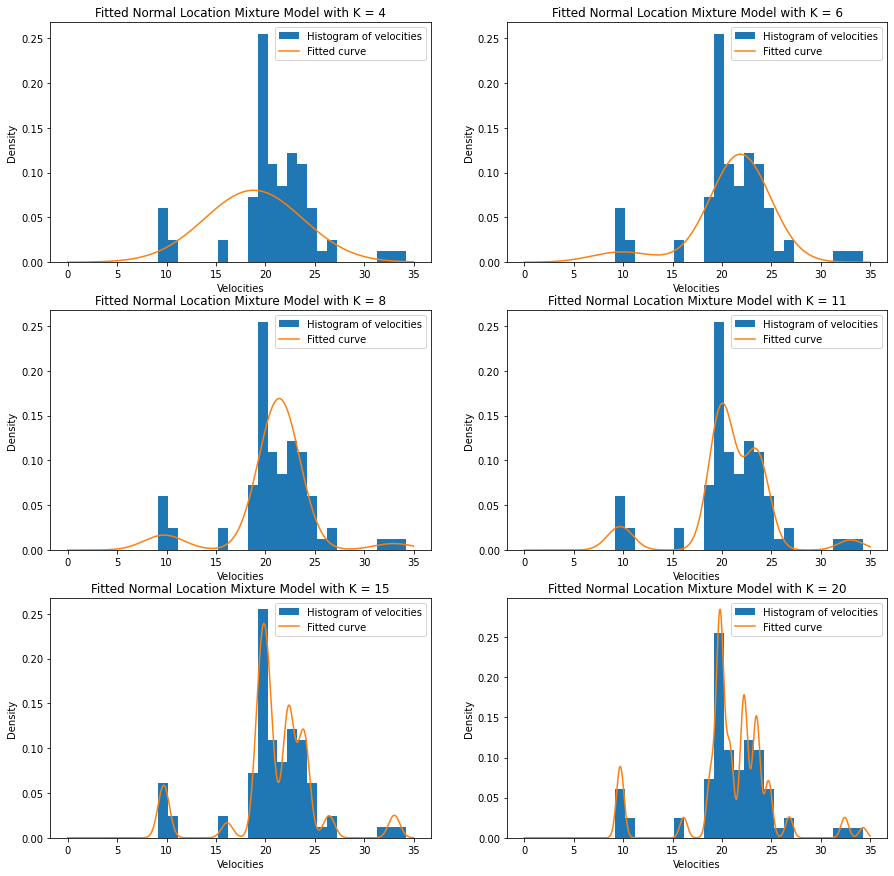
\includegraphics[width = 0.7\textwidth]{output.png}
  \caption{Normal Location Mixtures fitted for the Galaxies Dataset}
\end{figure}
\emph{b.} To calculate the AIC and BIC values, we make use of the following relations. Here, $\mathcal{L}(\theta)$ is the maximum value of the likelihood function for the model and p is the number of parameters, n is the number of data points.
\begin{equation}
  \nonumber
  \text{AIC (Akaike Information Criteria)} = 2\{-\mathcal{L}(\theta) + p\}
\end{equation}
\begin{equation}
  \nonumber
  \text{BIC (Bayesian Information Criteria)} = \{-2\mathcal{L}(\theta) + p \text{ log }n\}
\end{equation}
Using these relations, we can calculate the values of AIC and BIC for the models. Among a finite set of models; models with lower AIC and BIC are generally preferred.
\begin{center}
\begin{tabular}{ |c|c|c| }
  \hline
 \textbf{Model Components} & \textbf{AIC value} & \textbf{BIC value}\\
 \hline
 4 & 352.7817689704255 & 362.4086459594825 \\
 \hline
 6 & 335.5590562953825 & 349.999371778968 \\
 \hline
 8 & 380.22546857572144 & 399.4792225538355 \\
 \hline
 11 & 323.0554458958644 & 349.5293576157712 \\
 \hline
 15 & 357.3091456396654 & 393.40993434862924 \\
 \hline
 20 & 314.15244074768043 & 362.2868256929655 \\
 \hline
\end{tabular}
\end{center}
From this table, we can choose the model with 11 components as the best fit model, as both the AIC and BIC values are comparatively low. \\ \\
\noindent \emph{c.} Now, we fit normal location scale mixture models with form as follows.
\begin{equation}
  \nonumber
  y_{i} \overset{iid}{\sim} \sum_{k = 1}^{K} \pi_{k} \text{Normal}(y_{i} \text{ } | \text{ } \mu_{k}, \sigma_{k}^2)
\end{equation}
The EM Algorithm has been implemented in Python, and the steps to update the parameters of the normal location mixture distribution has been carried out according to the results taken from the lecture slides. (Pg. 36/96 - SDS-383C-F2022-M6-L3). To facilitate convergence, we keep the means fixed at initial values for the first 20 or so iterations and only update $\pi_{k}$'s and $\sigma_k$'s. After 20 or so iterations, we update all parameters. We arrive at the results for the fitted model as shown below.
\begin{figure}[H]
  \centering
  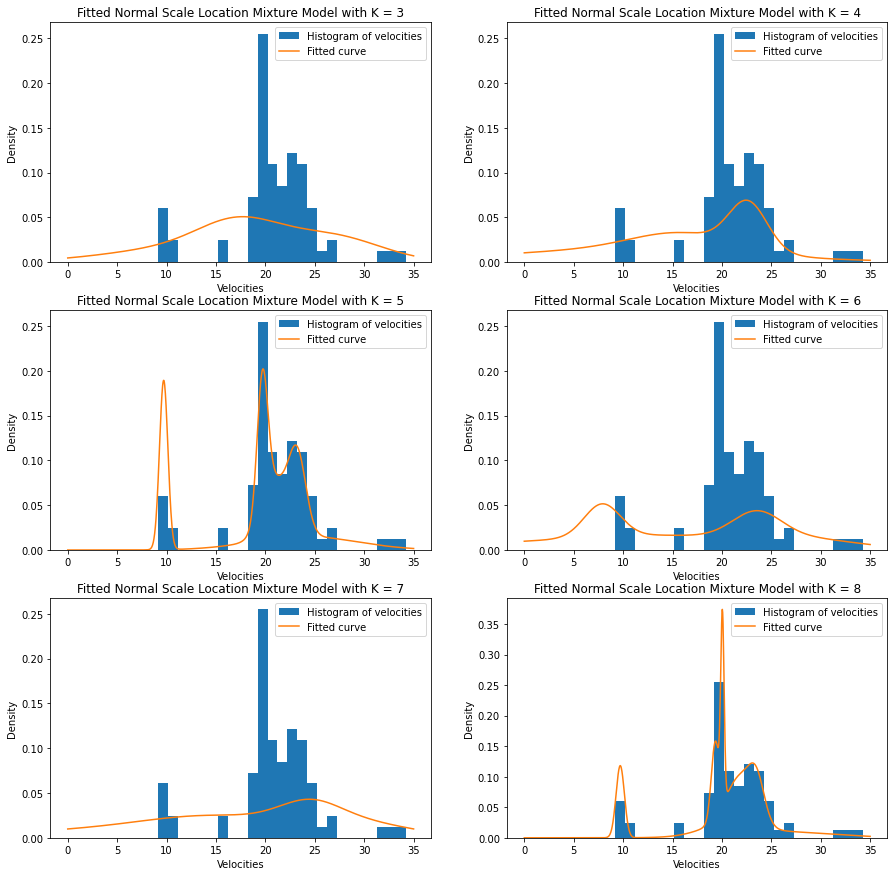
\includegraphics[width = 0.8\textwidth]{output2.png}
  \caption{Normal Location-Scale Mixtures fitted for the Galaxies Dataset}
\end{figure}
\emph{d.}Using the relations same as problem (b), we can calculate the values of AIC and BIC for the models. Among a finite set of models; models with lower AIC and BIC are generally preferred.
\begin{center}
\begin{tabular}{ |c|c|c| }
  \hline
 \textbf{Model Components} & \textbf{AIC value} & \textbf{BIC value}\\
 \hline
 3 & 536.0535205389705 & 543.2736782807632 \\
 \hline
 4 & 550.7503355546576 & 560.3772125437146 \\
 \hline
 5 & 379.0150026525681 & 391.0485988888894 \\
 \hline
 6 & 646.6301254358095& 661.0704409193951 \\
 \hline
 7 & 706.5958783561925 & 723.4429130870424 \\
 \hline
 8 & 433.5025155703568 & 452.75626954847087 \\
 \hline
\end{tabular}
\end{center}
From this table, we can choose the model with 5 components as the best fit model, as both the AIC and BIC values are comparatively low.
\emph{e.} In summary, we have fitted both the normal location and location scale mixtures using the EM algorithm. The EM is an iterative algorithm, that has 2 main steps.
\begin{equation}
  \nonumber
  \begin{aligned}
    \text{E - Step: Compute } Q(\theta, \theta^{(m)}) & = \mathbb{E}_{z \sim p(z | y, \theta^{m})}\text{ log }(p(y, z | \theta))\\
    \text{M - Step: Compute } \theta^{(m+1)} & = \underset{\theta}{\text{arg max }} Q(\theta, \theta^{(m)})
  \end{aligned}
\end{equation}
The convergence criteria has been specified to occur when the difference between the likelihood values between successive iterations becomes less than 0.0001. We see that in case of the normal location mixture model fitting, at larger values of K (=15,20) and in case of the normal location scale mixture model fitting, at larger values o K (=8), there are big spikes that accompany the fitted curve at certain points. This is due to overfitting, and is not ideal in choosing our best model. \\ \\
\emph{5.}\\ \\
\textbf{Solution: }
Now, we use the stochastic EM algorithm to fit location and location scale mixtures of normal to the galaxies dataset. The algorithm for updating the parameters using the stochastic EM algorithm is taken from the lecture slides (Pg. 96/96 - SDS-383C-F2022-M6-L3)
We obtain the following graphs for the Location and Location Scale Mixture respectively. The code is explained in detail in the comments in the code file. To facilitate convergence, we keep the means fixed at initial values for the first 20 or so iterations and only update $\pi_{k}$'s and $\sigma$ and $\sigma_{k}$'s. After 20 or so iterations, we update all parameters.
\begin{figure}[H]
  \centering
  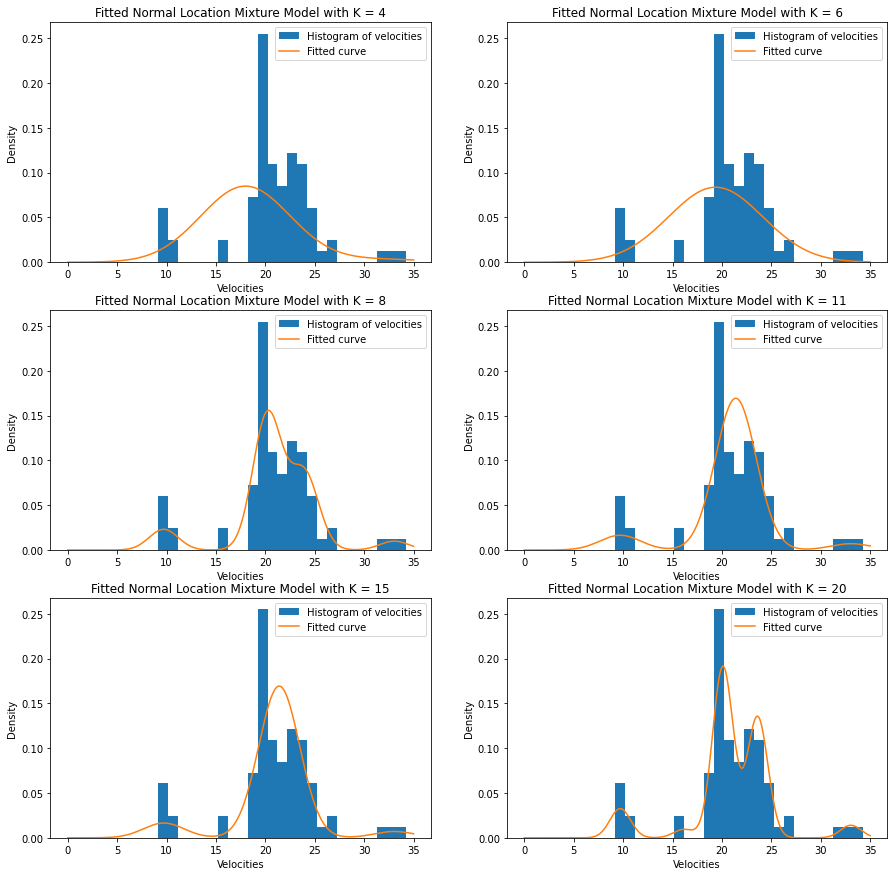
\includegraphics[width = 0.7\textwidth]{output5a.png}
  \caption{Normal Location Mixtures fitted for the Galaxies Dataset using the Stochastic EM Algorithm}
\end{figure}
The AIC and BIC values for the Normal Location mixture models fitted are tabulated as in correspondance to the relationships established in question 4b. The values are calculated as follows.
\begin{center}
\begin{tabular}{ |c|c|c| }
  \hline
 \textbf{Model Components} & \textbf{AIC value} & \textbf{BIC value}\\
 \hline
 4 & 370.06879972830274 & 383.63869188214187 \\
 \hline
 6 & 350.0827245349783 & 364.52304001856385 \\
 \hline
 8 & 321.1848947063752 & 335.1423880122533 \\
 \hline
 11 & 296.1514964613857 & 322.62540818129247 \\
 \hline
 15 & 304.1514964613857 & 340.2522851703495 \\
 \hline
 20 & 322.3315294430886 & 361.62052957897447 \\
 \hline
\end{tabular}
\end{center}
From this table, we can see that the best AIC and BIC values is given my the model with 11 components, as lower AIC and BIC values suggest better model perfomance.
\begin{figure}[H]
  \centering
  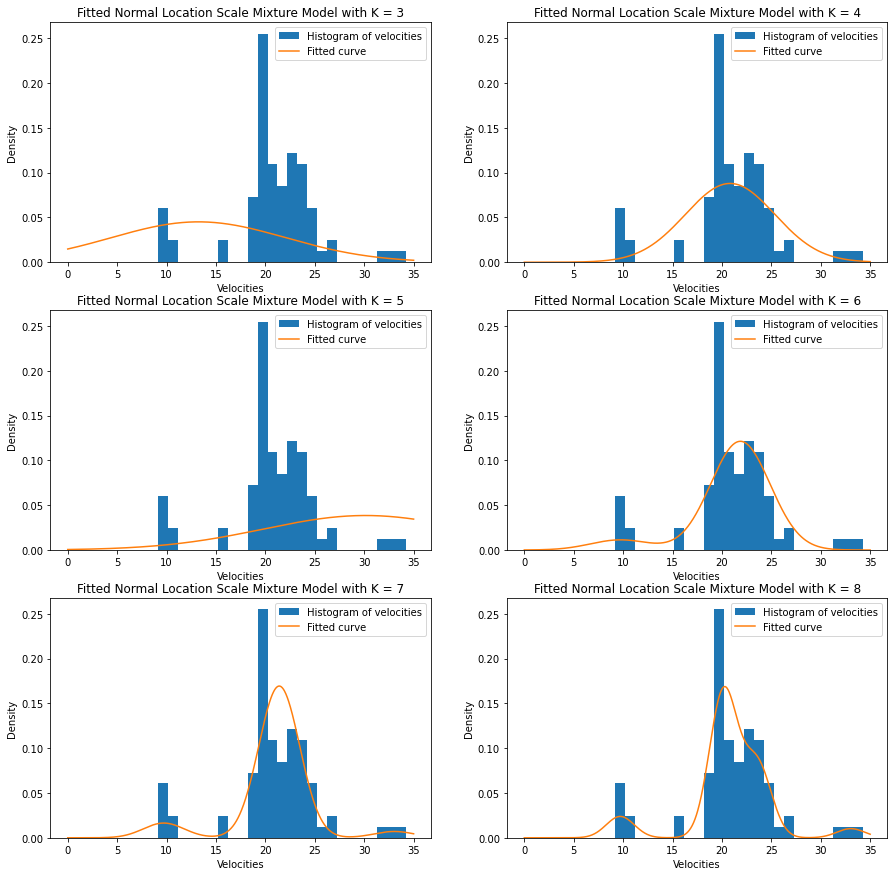
\includegraphics[width = 0.8\textwidth]{output5b.png}
  \caption{Normal Location - Scale Mixtures fitted for the Galaxies Dataset using the Stochastic EM Algorithm}
\end{figure}
\begin{center}
\begin{tabular}{ |c|c|c| }
  \hline
 \textbf{Model Components} & \textbf{AIC value} & \textbf{BIC value}\\
 \hline
 3 & 445.592073517817 & 452.8122312596098 \\
 \hline
 4 & 337.969862945876 & 347.596739934933 \\
 \hline
 5 & 475.3588669056884 & 487.39246314200966 \\
 \hline
 6 & 322.34396464344843 & 336.784280127034 \\
 \hline
 7 & 288.1514964613857 & 312.5526698778936 \\
 \hline
 8 & 312.3150580081916 & 346.4431622586945 \\
 \hline
\end{tabular}
\end{center}
From this table, we can see that the best AIC and BIC values is given my the model with 7 components, as lower AIC and BIC values suggest better model perfomance. We also observe that in the stochastic setting, the model is prone to quite a lot of error in the starting conditions. Also, the model fits the data well on a whole, which is expected from any stochastic algorithm. We also observe that the runtime and number of iterations taken to achieve convergence of the stochastic algorithm in both cases have been reduced significantly. \\ \\
\noindent \emph{6.} \\ \\
\emph{a.} Question 6 asks us to model a multivariate distribution of data. The dataset to be modelled is the ``Old Faithful Geyser'' dataset. This dataset was downloaded from the website \url{https://r-data.pmagunia.com/dataset/r-dataset-package-datasets-faithful}. The dataset consists of the waiting times between eruptions and the duration of the eruption for the Old Faithful geyser in Yellowstone National Park, Wyoming, USA. We desire to fit a Multivariate Normal Mixture Distribution with $K$ componenets of the form
\begin{equation}
  \nonumber
  \mathbf{y}_{1}, \dots, \mathbf{y}_{n} \overset{iid}{\sim} \sum_{k = 1}^{K} \pi_{k}\text{MVN}(\bm{\mu}_{k}, \bm{\Sigma}_{k})
\end{equation}
The EM Algorithm is used to fit these models. We start at an initial guess for the model parameters and iteratively update the values until convergence occurs. The convergence criteria is attained, when the log likelihood values between successive iterations has a tolerance of 0.0001. The equations to update the parameters of this model are implemented in Python, and the code has been explained in the comments. To speed up our calculations, we also have scaled down the values of each observation using the MinMaxScaler available in Python. We observe the following results. First, we plot the contour plots of the fitted densities superimposed over a scatterplot of the data points.
\begin{figure}[H]
  \centering
  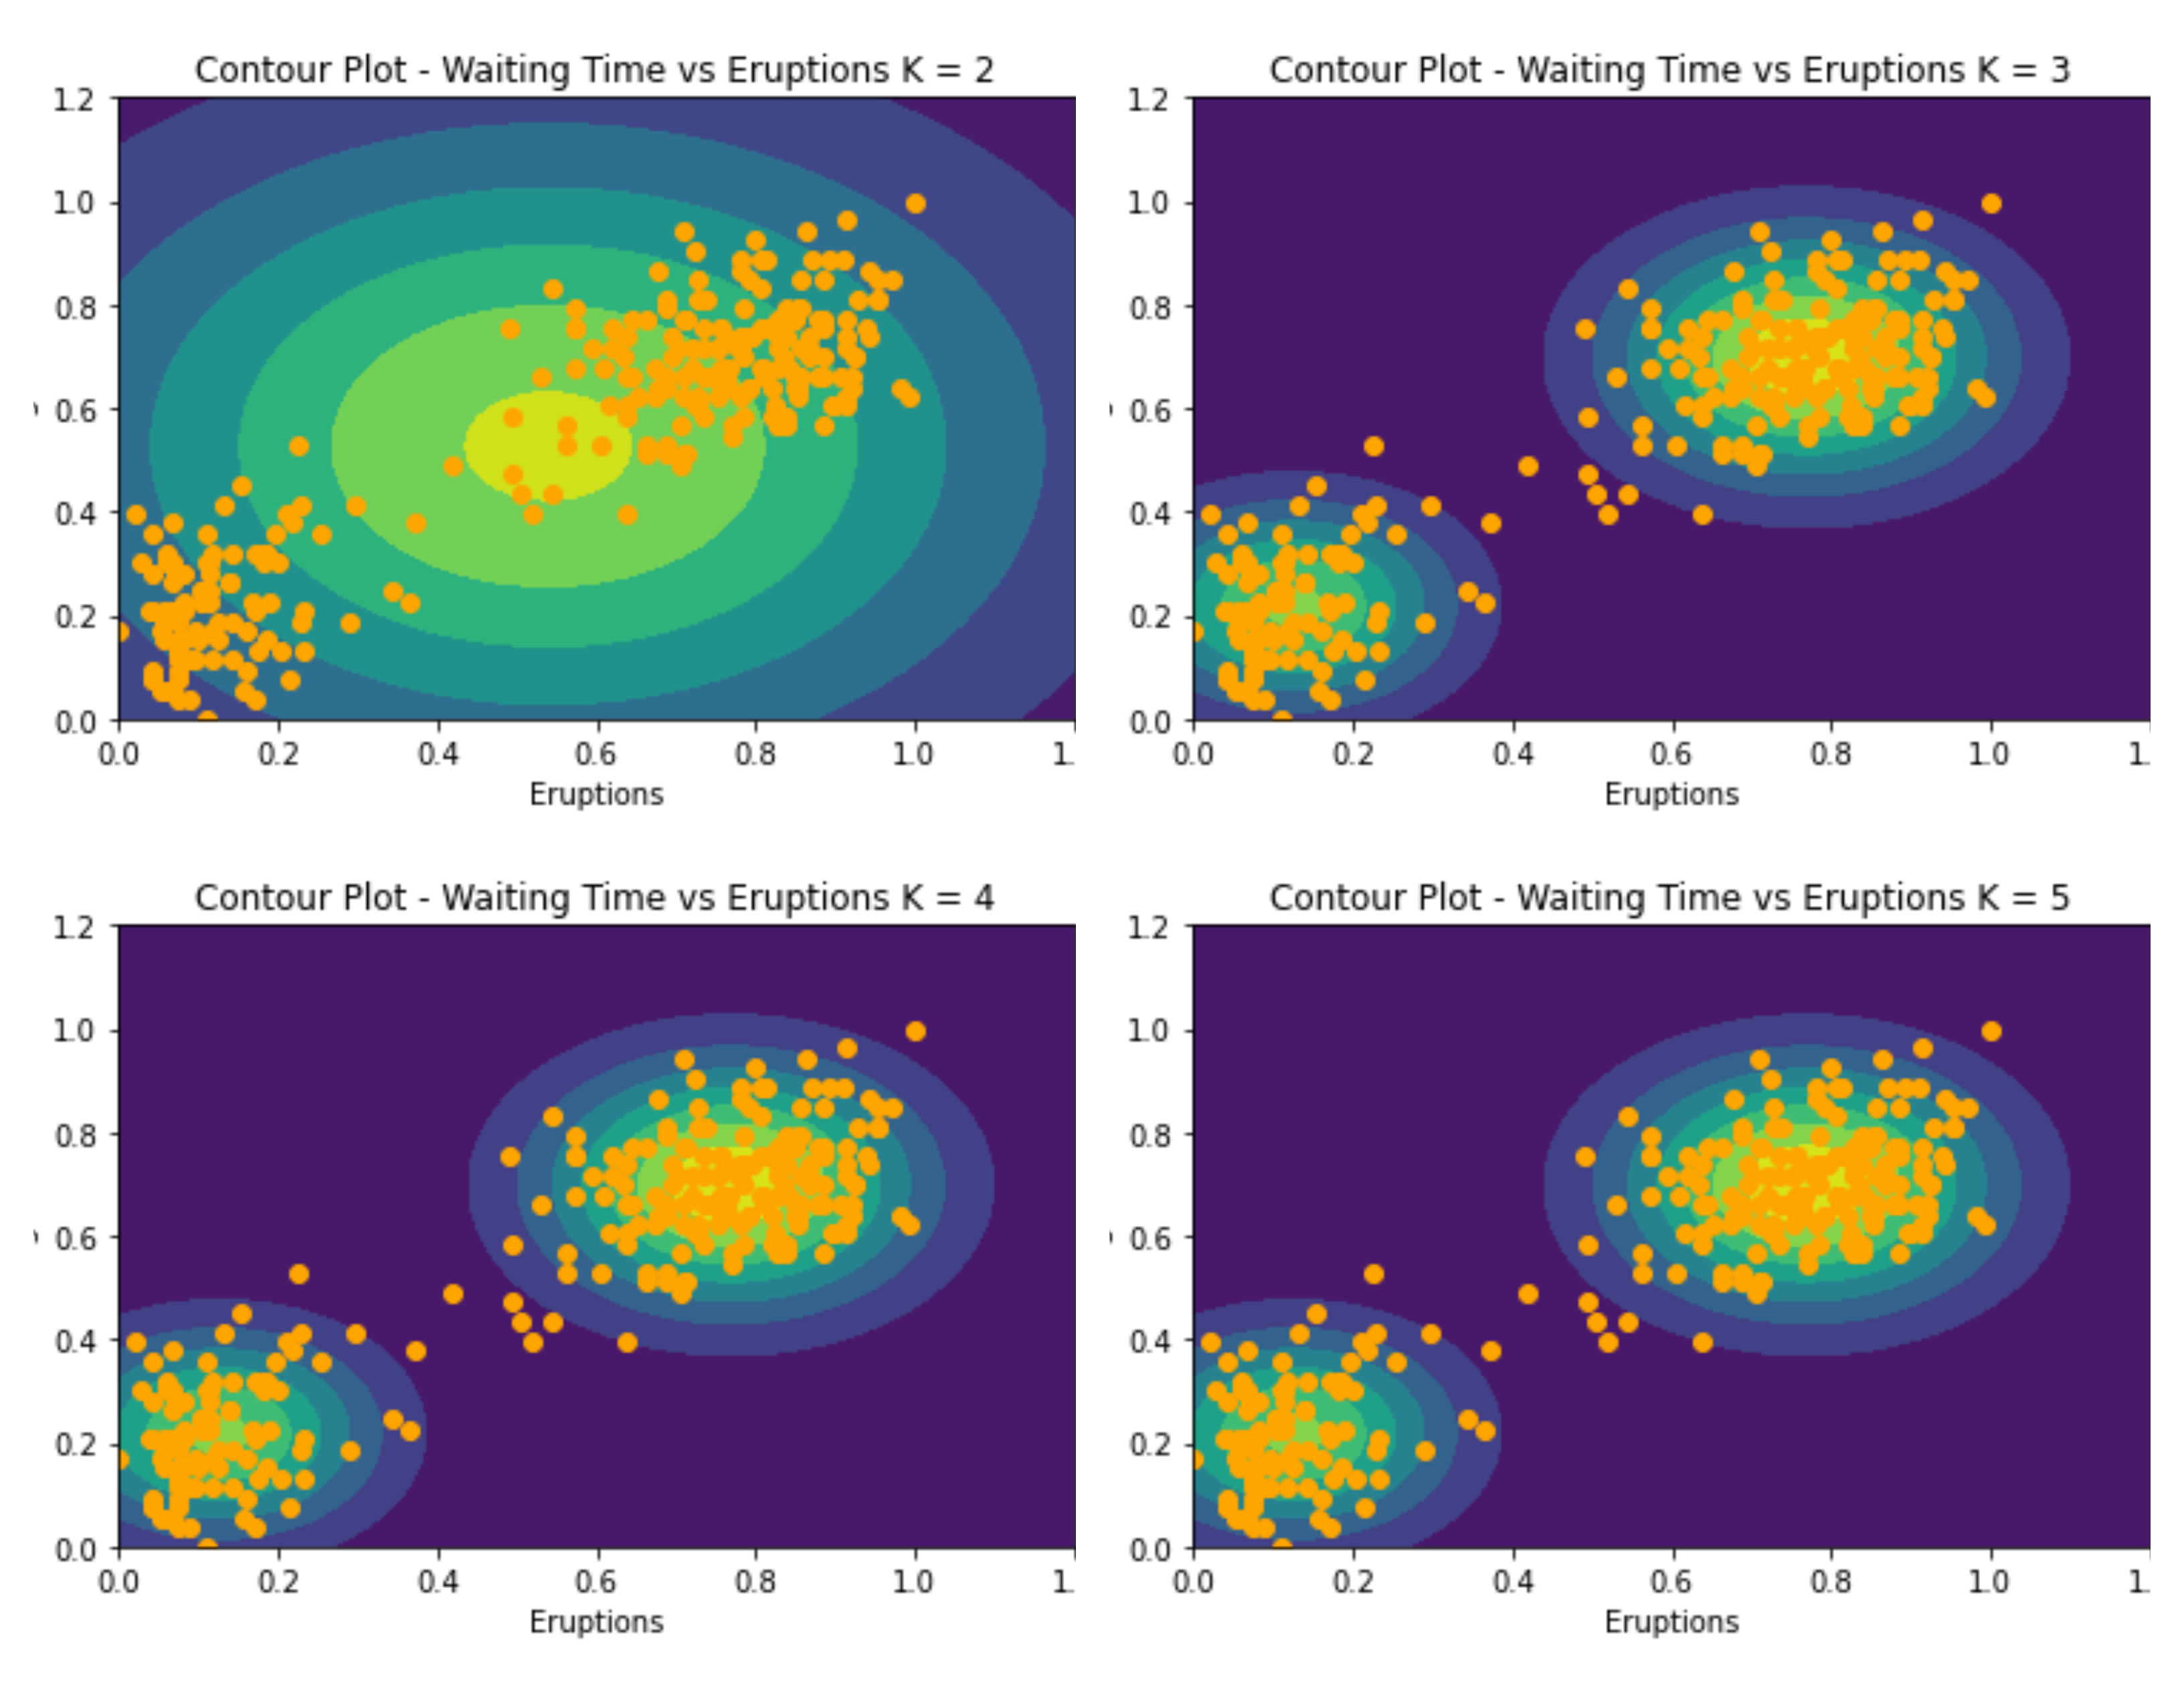
\includegraphics[width = 0.7\textwidth]{Contour Plots.png}
  \caption{Contours of the Multivariate Normal Mixtures fitted for the Old Faithful Geyser Dataset using the EM Algorithm}
\end{figure}
\noindent Further, we also plot the densities of these fitted mixture models in 3 dimensions to best visualize how the multivariate normal mixture functions.
\begin{figure}[H]
  \centering
  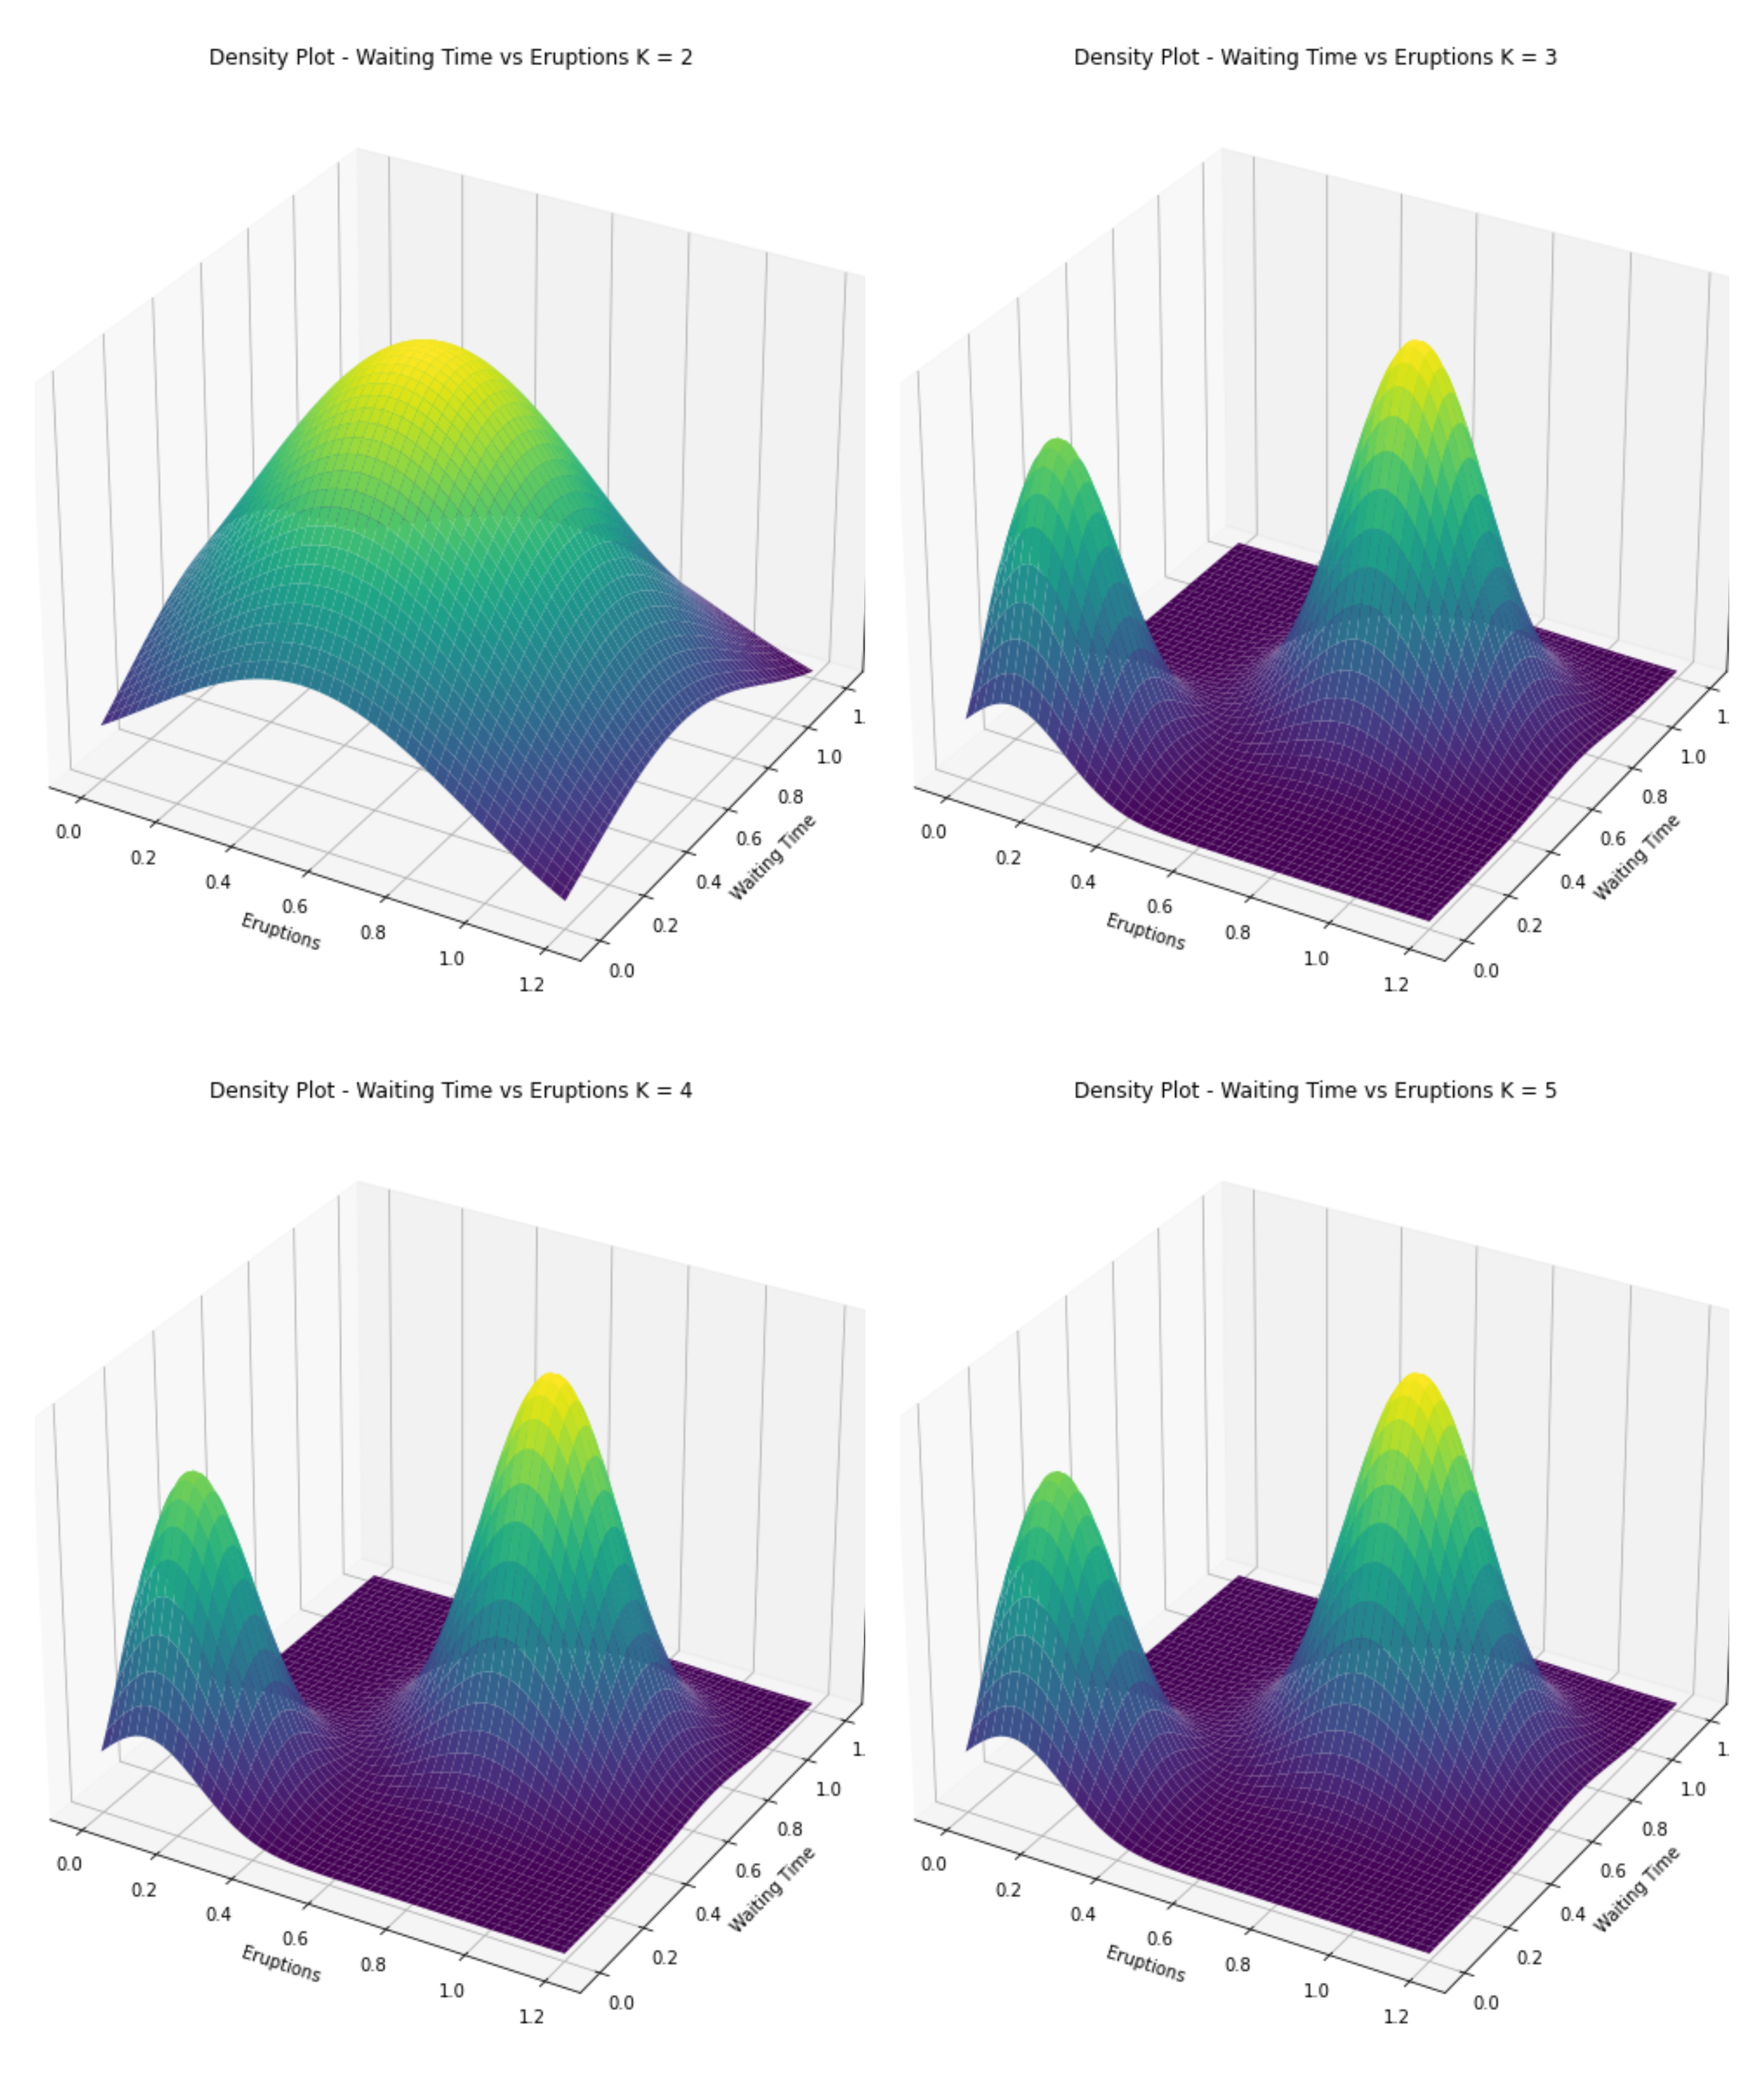
\includegraphics[width = 0.9\textwidth]{Density Plots.png}
  \caption{Densities of the Multivariate Normal Mixtures fitted for the Old Faithful Geyser Dataset using the EM Algorithm}
\end{figure}

\emph{b.} To identify the best model among the following mixtures, we make use of the AIC and BIC values. These values are calculated similar to question 4. That is,
\begin{equation}
  \nonumber
  \text{AIC (Akaike Information Criteria)} = 2\{-\mathcal{L}(\theta) + p\}
\end{equation}
\begin{equation}
  \nonumber
  \text{BIC (Bayesian Information Criteria)} = \{-2\mathcal{L}(\theta) + p \text{ log }n\}
\end{equation}
where p is the number of parameters, n is the number of data points, and $\mathcal{L}(\theta)$ is the log-likelihood value. Using these relations, we arrive at the following values for the AIC and BIC parameters.
\begin{center}
\begin{tabular}{ |c|c|c| }
  \hline
 \textbf{Model Components} & \textbf{AIC value} & \textbf{BIC value}\\
 \hline
 2 & -180.90964109228753 & 146.7566404232498 \\
 \hline
 3 & 136.87965618032885 & -173.69807017059864 \\
 \hline
 4 & -180.9112823836408 & 145.39070277577534 \\
 \hline
 5 & -180.932910192116 & -173.70826874375487 \\
 \hline
\end{tabular}
\end{center}
The lower the value for AIC and BIC, the better the fit of the model. The absolute value of the AIC or BIC value is not important. It can be positive or negative. From this table, we can conclude that therefore, the model with 5 components offers a better fit for our distribution.
\end{document}
